% Generated fragments require trusted human review before compilation.
% This binder never requests shell escape or runs external tools.
\documentclass[11pt]{article}
% Trusted shared apparatus. Requires LuaLaTeX; never use shell escape.
\usepackage{fontspec}
\defaultfontfeatures{Ligatures=TeX}
\IfFontExistsTF{Noto Serif}{\setmainfont{Noto Serif}}{%
  \IfFontExistsTF{DejaVu Serif}{\setmainfont{DejaVu Serif}}{%
    \IfFontExistsTF{Times New Roman}{\setmainfont{Times New Roman}}{%
      \PackageError{gelfand-binder}{No configured Cyrillic serif font installed}{Install Noto Serif or DejaVu Serif, or select an installed Cyrillic font.}%
    }%
  }%
}
\IfFontExistsTF{Noto Sans}{\setsansfont{Noto Sans}}{%
  \IfFontExistsTF{DejaVu Sans}{\setsansfont{DejaVu Sans}}{\setsansfont{Arial}}%
}
\IfFontExistsTF{Noto Sans Mono}{\setmonofont{Noto Sans Mono}}{%
  \IfFontExistsTF{DejaVu Sans Mono}{\setmonofont{DejaVu Sans Mono}}{\setmonofont{Courier New}}%
}
\usepackage[a4paper,margin=22mm]{geometry}
\usepackage{amsmath,amssymb,amsthm,mathtools}
\usepackage{xcolor}
\usepackage{tikz}
\usepackage{tikz-cd}
\usetikzlibrary{arrows.meta,positioning,calc}
\usepackage{hyperref}
\hypersetup{unicode=true,colorlinks=true,linkcolor=blue,pdftitle={Gelfand transcription binder}}
\newtheorem{theorem}{Theorem}
\newtheorem{lemma}{Lemma}
\newtheorem{proposition}{Proposition}
\newtheorem{corollary}{Corollary}
\theoremstyle{definition}
\newtheorem{definition}{Definition}
\newtheorem{example}{Example}
\theoremstyle{remark}
\newtheorem{remark}{Remark}
\setlength{\parindent}{0pt}
\setlength{\parskip}{0.55em}
\setlength{\emergencystretch}{3em}
\newcommand{\SourcePage}[2]{%
  \clearpage\phantomsection\label{#1:source-page}%
  \addcontentsline{toc}{subsection}{#1}%
  {\small\sffamily\color{blue!60!black}Source scan frame: #1; visible page/leaf label: #2}\par\medskip%
}
\newcommand{\Unclear}[3]{%
  \begingroup\color{orange!70!black}%
  [Unresolved reading #1/#2: #3]\endgroup%
}
\newcommand{\Incomplete}[3]{%
  \par\begingroup\color{red!65!black}\textbf{Incomplete #1/#2:} #3\endgroup\par%
}
\newcommand{\SourceFigure}[3]{%
  \par\begingroup\color{blue!60!black}\textbf{\hyperref[#1:source-page]{Source figure #1/#2}:} #3%
  \par\textit{Consult the authoritative scan at this locator.}\endgroup\par%
}



% Reader layout only. Original diplomatic text is retained verbatim.
\setlength{\parskip}{0.35em}
\setlength{\emergencystretch}{4em}
\renewcommand{\SourcePage}[2]{%
  \par\addvspace{1em}\phantomsection\label{#1:source-page}%
  \addcontentsline{toc}{subsection}{#1}%
  {\footnotesize\sffamily\color{blue!55!black}#1%
    \def\givenlabel{#2}\def\nolabel{unlabelled}%
    \ifx\givenlabel\nolabel\else\quad[номер в источнике: #2]\fi
  }\par\nobreak\smallskip%
}
\renewcommand{\Unclear}[3]{%
  \begingroup\color{orange!65!black}%
  \ifmmode\text{[неясно: #3]}\else[неясно: #3]\fi\endgroup%
}
\renewcommand{\Incomplete}[3]{%
  \par\begingroup\color{red!60!black}\textbf{Неразобранный фрагмент:} #3%
  \endgroup\par%
}
\renewcommand{\SourceFigure}[3]{%
  \par\begingroup\color{blue!55!black}\textbf{Рисунок:} #3%
  \par{\small\textit{Исходный рисунок: \hyperref[#1:source-page]{#1}, #2.}}%
  \endgroup\par%
}
\hypersetup{pdftitle={Семинар И. М. Гельфанда. Дипломатическая транскрипция},pdfauthor={},pdfsubject={Русское рабочее издание с отмеченными сомнительными чтениями}}

\usepackage[normalem]{ulem}
\usepackage{newunicodechar}
\usepackage{adjustbox}
\newfontfamily\SourceSymbolFont{Segoe UI Symbol}
\newfontfamily\SourceCJKFont{MS Gothic}
\let\DiplomaticMathUnderline\underline
\renewcommand{\underline}[1]{\ifmmode\DiplomaticMathUnderline{#1}\else\uline{#1}\fi}
\newunicodechar{→}{\ifmmode\text{{\SourceSymbolFont\char"2192}}\else{\SourceSymbolFont\char"2192}\fi}
\newunicodechar{⇒}{\ifmmode\text{{\SourceSymbolFont\char"21D2}}\else{\SourceSymbolFont\char"21D2}\fi}
\newunicodechar{∀}{\ifmmode\text{{\SourceSymbolFont\char"2200}}\else{\SourceSymbolFont\char"2200}\fi}
\newunicodechar{∂}{\ifmmode\text{{\SourceSymbolFont\char"2202}}\else{\SourceSymbolFont\char"2202}\fi}
\newunicodechar{∈}{\ifmmode\text{{\SourceSymbolFont\char"2208}}\else{\SourceSymbolFont\char"2208}\fi}
\newunicodechar{∌}{\ifmmode\text{{\SourceSymbolFont\char"220C}}\else{\SourceSymbolFont\char"220C}\fi}
\newunicodechar{√}{\ifmmode\text{{\SourceSymbolFont\char"221A}}\else{\SourceSymbolFont\char"221A}\fi}
\newunicodechar{∞}{\ifmmode\text{{\SourceSymbolFont\char"221E}}\else{\SourceSymbolFont\char"221E}\fi}
\newunicodechar{∧}{\ifmmode\text{{\SourceSymbolFont\char"2227}}\else{\SourceSymbolFont\char"2227}\fi}
\newunicodechar{∩}{\ifmmode\text{{\SourceSymbolFont\char"2229}}\else{\SourceSymbolFont\char"2229}\fi}
\newunicodechar{∪}{\ifmmode\text{{\SourceSymbolFont\char"222A}}\else{\SourceSymbolFont\char"222A}\fi}
\newunicodechar{∫}{\ifmmode\text{{\SourceSymbolFont\char"222B}}\else{\SourceSymbolFont\char"222B}\fi}
\newunicodechar{∴}{\ifmmode\text{{\SourceSymbolFont\char"2234}}\else{\SourceSymbolFont\char"2234}\fi}
\newunicodechar{∼}{\ifmmode\text{{\SourceSymbolFont\char"223C}}\else{\SourceSymbolFont\char"223C}\fi}
\newunicodechar{≈}{\ifmmode\text{{\SourceSymbolFont\char"2248}}\else{\SourceSymbolFont\char"2248}\fi}
\newunicodechar{≠}{\ifmmode\text{{\SourceSymbolFont\char"2260}}\else{\SourceSymbolFont\char"2260}\fi}
\newunicodechar{≤}{\ifmmode\text{{\SourceSymbolFont\char"2264}}\else{\SourceSymbolFont\char"2264}\fi}
\newunicodechar{≥}{\ifmmode\text{{\SourceSymbolFont\char"2265}}\else{\SourceSymbolFont\char"2265}\fi}
\newunicodechar{⊕}{\ifmmode\text{{\SourceSymbolFont\char"2295}}\else{\SourceSymbolFont\char"2295}\fi}
\newunicodechar{⊗}{\ifmmode\text{{\SourceSymbolFont\char"2297}}\else{\SourceSymbolFont\char"2297}\fi}
\newunicodechar{①}{\ifmmode\text{{\SourceSymbolFont\char"2460}}\else{\SourceSymbolFont\char"2460}\fi}
\newunicodechar{②}{\ifmmode\text{{\SourceSymbolFont\char"2461}}\else{\SourceSymbolFont\char"2461}\fi}
\newunicodechar{③}{\ifmmode\text{{\SourceSymbolFont\char"2462}}\else{\SourceSymbolFont\char"2462}\fi}
\newunicodechar{④}{\ifmmode\text{{\SourceSymbolFont\char"2463}}\else{\SourceSymbolFont\char"2463}\fi}
\newunicodechar{Ⓗ}{\ifmmode\text{{\SourceSymbolFont\char"24BD}}\else{\SourceSymbolFont\char"24BD}\fi}
\newunicodechar{〃}{\ifmmode\text{{\SourceCJKFont\char"3003}}\else{\SourceCJKFont\char"3003}\fi}


% Reader revision 3. Annotation wording and candidates remain unchanged.
\usetikzlibrary{shapes.geometric,decorations.pathreplacing,decorations.markings,patterns,fit}
\newsavebox{\ReaderAnnotationBox}
\newcommand{\ReaderAnnotation}[1]{%
  \sbox{\ReaderAnnotationBox}{[неясно: #1]}%
  \ifdim\wd\ReaderAnnotationBox>.70\linewidth
    \parbox[t]{.70\linewidth}{\raggedright[неясно: #1]}%
  \else\usebox{\ReaderAnnotationBox}\fi%
}
\ExplSyntaxOn
\cs_new_protected:Npn \reader_unclear_candidate:n #1
 {
  \tl_set:Nx \l_tmpa_tl { \tl_to_str:n {#1} }
  % Text explicitly guarded inside a mathematical candidate remains math-safe.
  \regex_replace_all:nnN { \\(?:text|textrm|textnormal|textbf|operatorname)\s*\{[^{}]*\} } { } \l_tmpa_tl
  \regex_match:nVTF { [\x{0400}-\x{052F}] | \$ } \l_tmpa_tl
   { \ifmmode \text{\ReaderAnnotation{#1}} \else \ReaderAnnotation{#1} \fi }
   {
    \ifmmode
      [\text{неясно:~}#1]
    \else
      \regex_match:nVTF { [_^] | \\ } \l_tmpa_tl
       { \ensuremath{[\text{неясно:~}#1]} }
       { \ReaderAnnotation{#1} }
    \fi
   }
 }
\RenewDocumentCommand \Unclear { m m m }
 { \begingroup\color{orange!65!black}\reader_unclear_candidate:n{#3}\endgroup }
\ExplSyntaxOff
\newsavebox{\ReaderIncompleteBox}
\newcommand{\ReaderIncompleteNote}[1]{%
 \sbox{\ReaderIncompleteBox}{\textbf{Неразобранный фрагмент:} #1}%
 \ifdim\wd\ReaderIncompleteBox>.70\linewidth
  \parbox[t]{.70\linewidth}{\raggedright\textbf{Неразобранный фрагмент:} #1}%
 \else\usebox{\ReaderIncompleteBox}\fi%
}
\renewcommand{\Incomplete}[3]{%
 \ifmmode\text{\color{red!60!black}\ReaderIncompleteNote{#3}}%
 \else\par\begingroup\color{red!60!black}\textbf{Неразобранный фрагмент:} #3\endgroup\par\fi%
}
% Ragged right avoids stretching long untranslated abbreviations into margins.
\AtBeginDocument{\raggedright}
\newunicodechar{А}{\ifmmode\text{\char"410\relax}\else\char"410\relax\fi}
\newunicodechar{Б}{\ifmmode\text{\char"411\relax}\else\char"411\relax\fi}
\newunicodechar{В}{\ifmmode\text{\char"412\relax}\else\char"412\relax\fi}
\newunicodechar{Г}{\ifmmode\text{\char"413\relax}\else\char"413\relax\fi}
\newunicodechar{Д}{\ifmmode\text{\char"414\relax}\else\char"414\relax\fi}
\newunicodechar{Е}{\ifmmode\text{\char"415\relax}\else\char"415\relax\fi}
\newunicodechar{Ж}{\ifmmode\text{\char"416\relax}\else\char"416\relax\fi}
\newunicodechar{З}{\ifmmode\text{\char"417\relax}\else\char"417\relax\fi}
\newunicodechar{И}{\ifmmode\text{\char"418\relax}\else\char"418\relax\fi}
\newunicodechar{Й}{\ifmmode\text{\char"419\relax}\else\char"419\relax\fi}
\newunicodechar{К}{\ifmmode\text{\char"41A\relax}\else\char"41A\relax\fi}
\newunicodechar{Л}{\ifmmode\text{\char"41B\relax}\else\char"41B\relax\fi}
\newunicodechar{М}{\ifmmode\text{\char"41C\relax}\else\char"41C\relax\fi}
\newunicodechar{Н}{\ifmmode\text{\char"41D\relax}\else\char"41D\relax\fi}
\newunicodechar{О}{\ifmmode\text{\char"41E\relax}\else\char"41E\relax\fi}
\newunicodechar{П}{\ifmmode\text{\char"41F\relax}\else\char"41F\relax\fi}
\newunicodechar{Р}{\ifmmode\text{\char"420\relax}\else\char"420\relax\fi}
\newunicodechar{С}{\ifmmode\text{\char"421\relax}\else\char"421\relax\fi}
\newunicodechar{Т}{\ifmmode\text{\char"422\relax}\else\char"422\relax\fi}
\newunicodechar{У}{\ifmmode\text{\char"423\relax}\else\char"423\relax\fi}
\newunicodechar{Ф}{\ifmmode\text{\char"424\relax}\else\char"424\relax\fi}
\newunicodechar{Х}{\ifmmode\text{\char"425\relax}\else\char"425\relax\fi}
\newunicodechar{Ц}{\ifmmode\text{\char"426\relax}\else\char"426\relax\fi}
\newunicodechar{Ч}{\ifmmode\text{\char"427\relax}\else\char"427\relax\fi}
\newunicodechar{Ш}{\ifmmode\text{\char"428\relax}\else\char"428\relax\fi}
\newunicodechar{Щ}{\ifmmode\text{\char"429\relax}\else\char"429\relax\fi}
\newunicodechar{Ъ}{\ifmmode\text{\char"42A\relax}\else\char"42A\relax\fi}
\newunicodechar{Ы}{\ifmmode\text{\char"42B\relax}\else\char"42B\relax\fi}
\newunicodechar{Ь}{\ifmmode\text{\char"42C\relax}\else\char"42C\relax\fi}
\newunicodechar{Э}{\ifmmode\text{\char"42D\relax}\else\char"42D\relax\fi}
\newunicodechar{Ю}{\ifmmode\text{\char"42E\relax}\else\char"42E\relax\fi}
\newunicodechar{Я}{\ifmmode\text{\char"42F\relax}\else\char"42F\relax\fi}
\newunicodechar{а}{\ifmmode\text{\char"430\relax}\else\char"430\relax\fi}
\newunicodechar{б}{\ifmmode\text{\char"431\relax}\else\char"431\relax\fi}
\newunicodechar{в}{\ifmmode\text{\char"432\relax}\else\char"432\relax\fi}
\newunicodechar{г}{\ifmmode\text{\char"433\relax}\else\char"433\relax\fi}
\newunicodechar{д}{\ifmmode\text{\char"434\relax}\else\char"434\relax\fi}
\newunicodechar{е}{\ifmmode\text{\char"435\relax}\else\char"435\relax\fi}
\newunicodechar{ж}{\ifmmode\text{\char"436\relax}\else\char"436\relax\fi}
\newunicodechar{з}{\ifmmode\text{\char"437\relax}\else\char"437\relax\fi}
\newunicodechar{и}{\ifmmode\text{\char"438\relax}\else\char"438\relax\fi}
\newunicodechar{й}{\ifmmode\text{\char"439\relax}\else\char"439\relax\fi}
\newunicodechar{к}{\ifmmode\text{\char"43A\relax}\else\char"43A\relax\fi}
\newunicodechar{л}{\ifmmode\text{\char"43B\relax}\else\char"43B\relax\fi}
\newunicodechar{м}{\ifmmode\text{\char"43C\relax}\else\char"43C\relax\fi}
\newunicodechar{н}{\ifmmode\text{\char"43D\relax}\else\char"43D\relax\fi}
\newunicodechar{о}{\ifmmode\text{\char"43E\relax}\else\char"43E\relax\fi}
\newunicodechar{п}{\ifmmode\text{\char"43F\relax}\else\char"43F\relax\fi}
\newunicodechar{р}{\ifmmode\text{\char"440\relax}\else\char"440\relax\fi}
\newunicodechar{с}{\ifmmode\text{\char"441\relax}\else\char"441\relax\fi}
\newunicodechar{т}{\ifmmode\text{\char"442\relax}\else\char"442\relax\fi}
\newunicodechar{у}{\ifmmode\text{\char"443\relax}\else\char"443\relax\fi}
\newunicodechar{ф}{\ifmmode\text{\char"444\relax}\else\char"444\relax\fi}
\newunicodechar{х}{\ifmmode\text{\char"445\relax}\else\char"445\relax\fi}
\newunicodechar{ц}{\ifmmode\text{\char"446\relax}\else\char"446\relax\fi}
\newunicodechar{ч}{\ifmmode\text{\char"447\relax}\else\char"447\relax\fi}
\newunicodechar{ш}{\ifmmode\text{\char"448\relax}\else\char"448\relax\fi}
\newunicodechar{щ}{\ifmmode\text{\char"449\relax}\else\char"449\relax\fi}
\newunicodechar{ъ}{\ifmmode\text{\char"44A\relax}\else\char"44A\relax\fi}
\newunicodechar{ы}{\ifmmode\text{\char"44B\relax}\else\char"44B\relax\fi}
\newunicodechar{ь}{\ifmmode\text{\char"44C\relax}\else\char"44C\relax\fi}
\newunicodechar{э}{\ifmmode\text{\char"44D\relax}\else\char"44D\relax\fi}
\newunicodechar{ю}{\ifmmode\text{\char"44E\relax}\else\char"44E\relax\fi}
\newunicodechar{я}{\ifmmode\text{\char"44F\relax}\else\char"44F\relax\fi}
\newunicodechar{Ё}{\ifmmode\text{\char"401\relax}\else\char"401\relax\fi}
\newunicodechar{ё}{\ifmmode\text{\char"451\relax}\else\char"451\relax\fi}

\begin{document}
\begin{center}
{\Large Семинар И. М. Гельфанда}\par\medskip
{\LARGE Дипломатическая транскрипция}\par\bigskip
{\large Рабочее русское издание}\par\medskip
{\large Том 17 из 34. Архивная глава 017}\par\bigskip
Кадры GELFAND-P000900 -- GELFAND-P000918\par

\end{center}
\medskip
Сокращения, отменённые записи и сомнительные чтения сохранены.
Неразобранные фрагменты отмечены в тексте. Математические утверждения
источника переданы без молчаливых исправлений.

Это рабочее издание: сверка с рукописью продолжается. В текущем комплекте
учтены 1503 из 1527 кадров; 24 кадра пока представлены явными указателями
отсутствующего возврата. Полный журнал чтений и происхождения данных
сохранён в основном рабочем переплёте.

Границы кадров показаны небольшими синими указателями; печатный текст
продолжается без обязательного разрыва страницы после каждого кадра.
\bigskip\hrule\bigskip
\SourcePage{GELFAND-P000900}{3}
% Original 2432 x 3471. All coordinates below refer to original source pixels.
% Full-frame inspection, then bands (130,35,2290,310), (115,300,2190,670),
% (140,680,2220,1215), (170,1280,2260,1845), (140,1920,2200,2580),
% (135,2620,2200,3471). Further 3x--10x review regions are recorded in the ledger.
\underline{\underline{21.1.80.}}\qquad \underline{Сем Гельфанда.}

\underline{\underline{А. Мигдал.}}\qquad
\underline{О новом подходе к калибровочным теориям.}

Это новый язык, более адекватный для описания сильных взаимодействий.

\underline{Старый язык:}\quad $SU(N)$

поля
\begin{equation*}
 A_\mu(x)=\sum_{a=1}^{N^2-1}T_a A_\mu^a,
 \qquad T_a\text{ — генераторы }SU(N).\tag{1}
\end{equation*}
[Под $A_\mu(x)$: (связность).]

Язык был бы адекватен, если бы поля были близки к $0$ или другому
классич. решению (не так сильно флуктуировали).

Нужно рассматривать.
\begin{equation*}
 \Psi(c)=\operatorname{Tr}\,p\exp\left(\oint A\,dx\right),\tag{2}
\end{equation*}
где $c$ — петля,
\begin{equation*}
 p\exp\left(\oint A\,dx\right)=\prod\bigl(1+A_\alpha(x)\,dx\bigr)\tag{3}
\end{equation*}
\Unclear{GELFAND-P000900}{equation03-differential}{В (3) виден $A_\alpha(x)\,dx$; индекс при $dx$ не виден.}

Без следа в (2) — [Зачёркнуто:
\Unclear{GELFAND-P000900}{cancel-before-covariant}{ков.?}] ковар. величина.
Оказывается можно ограничиться тем, что получится, если взять след.

Итак, нужно петлевое пр-во.

Неинвар. величины в квант. теории получаются равными $0$.

\begin{center}— $\bullet$ —\end{center}

\underline{И.М.Г.} Суть дела: представление гр. путей опред. характером.

% Separator source box (755,1360,1015,1425), independently reviewed at 6x.
\begin{center}— $\bullet$ —\end{center}

Здесь речь идёт о наинизшем характере.

Паралл. перенос:
\begin{equation*}
 \frac{dF}{dx}=AF\quad\Rightarrow\quad F=C e^{\int A\,dx}
\end{equation*}
для матриц интеграл упоряд.

Группа путей.
\SourceFigure{GELFAND-P000900}{path-retracing-sketch}{Дугообразный путь: утолщённая точка слева внизу, две близкие ветви справа и противоположно направленные наконечники наверху и справа; точное разделение ветвей требует проверки.}
сокращаем пути туда-обратно.

\begin{center}— $\bullet$ —\end{center}

Пусть $A_\mu$ удовлетв. классическим ур-ям дв-ния:
\begin{equation*}
 \nabla_\mu F_{\mu\nu}=0,\tag{4}
\end{equation*}
где
\begin{equation*}
 F_{\mu\nu}=\partial_\mu A_\nu-\partial_\nu A_\mu+[A_\mu,A_\nu]\tag{5}
\end{equation*}
(кривизна связности)

Напишем условие, к-рому удовлетворяет в этом случае функция $\Psi(c)$.

(6)
\SourceFigure{GELFAND-P000900}{attached-loop-sketch}{Большой вертикальный овал с маленькой петелькой слева; около места присоединения справа от линии написано $x$. У стыка виден направленный вверх утолщённый штрих; его чтение как стрелки требует проверки.}
$c+\delta\sigma_{\mu\nu}$,\quad $\delta\sigma_{\mu\nu}$ — площадь
\quad (пристроили петельку к контуру $c$)

\begin{equation*}
 \frac{\delta\Psi}{\delta\sigma_{\mu\nu}}
 =\operatorname{Tr}\left(\hat p F_{\mu\nu}\exp\left(\oint A\,dx\right)\right)\tag{7}
\end{equation*}

Докажем (7): имеем
\begin{equation*}
 \Psi(c_x+\delta c_x)-\Psi(c)
 \equiv\frac{\delta\Psi}{\delta\sigma_{\mu\nu}}
 \int_{\delta c}x_\mu'\,dx_\nu\tag{8}
\end{equation*}
\Unclear{GELFAND-P000900}{equation08-arguments}{В (8) $c_x$ содержит густую правку; аргумент второго $\Psi$ читается как $c$ / $\delta$ и также переписан.}
\Unclear{GELFAND-P000900}{equation08-prime}{В (8) над $x_\mu$ виден отдельный вертикальный штрих: $x_\mu'$ / $x_\mu$ с посторонним штрихом.}

\underline{Функционал типа Стокса.} если вариация пропорц площади
(это не всегда так. напр, для длины)

\SourcePage{GELFAND-P000901}{unlabelled}
\Unclear{GELFAND-P000901}{upper-left-mark}{Неясная помета на верхнем левом поле.}

В абелевом случае это теорема Стокса.
\begin{equation*}
\oint_{\delta C} A_\alpha\,dx_\alpha
=\int_{\delta S} F_{\alpha\beta}\,d\sigma_{\alpha\beta}.
\tag{9}
\end{equation*}

(\Unclear{GELFAND-P000901}{upper-parenthesis-word}{рассм. или расск.}
раб. с \underline{Макеенко} и использ. работы авторов
Мандельстам, Намбу, Поляков)

$\hat p$ в (7) действ. и на $F_{\mu\nu}$ и на $\exp$.

$F_{\mu\nu}(x)$ ставится туда, где точка $x$

Или:
\begin{equation*}
\frac{\delta\Psi}{\delta\sigma_{\mu\nu}}
=\operatorname{Tr}\bigl(F_{\mu\nu}(x)\,p\exp(\int_x^x A\,dx)\bigr)
\tag{10}
\end{equation*}
\begin{center}
\begin{adjustbox}{max width=\linewidth}
\begin{tikzpicture}
\node at (0,0) {на кривой появилась};
\node at (5.2,0) {\Unclear{GELFAND-P000901}{equation-10-note}{отм.} точка $x$};
\draw[->] (0.3,0.3) -- (0.7,1.0);
\end{tikzpicture}
\end{adjustbox}
\end{center}

\underline{Док-во} (7):
\begin{equation*}
\prod(1+A(x)\,dx)
=\prod\bigl(1+dx_\mu(A_\mu(x_0)+\frac{\partial}{\partial x_\mu})\bigr)
=\prod[1+dx_\mu\nabla_\mu(x_0)]
\tag{11}
\end{equation*}
\begin{center}
\begin{adjustbox}{max width=\linewidth}
\begin{tikzpicture}[x=1cm,y=1cm]
\node at (-0.6,0) {$x_0$};
\draw (0,0) .. controls (0.3,0.12) and (0.6,0.12) .. (0.9,0)
.. controls (1.2,-0.09) and (1.5,-0.1) .. (1.9,0)
.. controls (2.3,0.08) and (2.5,-0.02) .. (2.9,0.02);
\draw (0,-0.14)--(0,0.12);
\draw (0.3,-0.1)--(0.3,0.2);
\draw (0.65,-0.1)--(0.65,0.21);
\draw (1,-0.12)--(1,0.17);
\draw (1.35,-0.14)--(1.35,0.1);
\draw (1.7,-0.12)--(1.7,0.12);
\draw (2.02,-0.1)--(2.02,0.14);
\draw (2.34,-0.1)--(2.34,0.14);
\draw (2.62,-0.1)--(2.62,0.13);
\draw (2.77,-0.1)--(2.77,0.13);
\draw (2.9,-0.12)--(2.9,0.16);
\node at (3.22,-0.12) {$x_1$};
\node at (1,-0.6) {нач. точка};
\node at (7.3,-0.2) {опред. $\nabla_\mu=A_\mu(x_0)+\dfrac{\partial}{\partial x_\mu}$};
\draw[->] (5.45,0.15)--(5.6,0.7);
\end{tikzpicture}
\end{adjustbox}
\end{center}

$dx_\mu\dfrac{\partial}{\partial x_\mu}$ \underline{сдвигает аргумент}

\begin{center}
\begin{adjustbox}{max width=\linewidth}
\begin{tikzpicture}[x=1cm,y=1cm]
\node at (-2,0.4) {(12)};
\draw (0.8,0.8) .. controls (1.5,2.2) and (3.1,1.7) .. (2.3,-0.5)
.. controls (1.8,-1.3) and (1.0,-0.1) .. (0.8,0.55);
\draw[->] (0.8,0.8)--(-0.4,0.55);
\draw[->] (-0.4,0.55)--(-0.4,-0.3);
\draw[->] (-0.4,-0.3)--(0.8,-0.1);
\draw[->] (0.8,-0.1)--(0.8,0.55);
\node at (0.1,1.0) {$\mu$};
\node at (-0.75,0.1) {$\nu$};
\node at (0.2,-0.62) {$\mu$};
\node at (0.48,0.22) {$\nu$};
\node at (6.4,0.25) {--- рассм. такую вариацию};
\end{tikzpicture}
\end{adjustbox}
\end{center}

\begin{equation*}
\begin{aligned}
&(1+dx_\mu\nabla_\mu)(1+dx_\nu\nabla_\nu)
(1-dx_\mu\nabla_\mu)(1-dx_\nu\nabla_\nu)=\\
&\qquad=1+dx_\mu\wedge dx_\nu[\nabla_\mu,\nabla_\nu]
\end{aligned}
\tag{13}
\end{equation*}

(здесь все $\nabla_\mu$ относятся к нач. точке)

Пусть 2 отрезка:
\begin{center}
\begin{adjustbox}{max width=\linewidth}
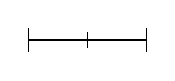
\begin{tikzpicture}
\draw (0,0)--(1.5,0);
\draw (0,-0.15)--(0,0.15);
\draw (0.75,-0.1)--(0.75,0.1);
\draw (1.5,-0.15)--(1.5,0.15);
\end{tikzpicture}
\end{adjustbox}
\end{center}
\begin{equation*}
\begin{aligned}
&(1+A(x_0)\,dx_1)(1+A(x_0+dx_1)\,dx_2)=\\
&=[1+dx_1(A(x_0)+\frac{\partial}{\partial x_0})](1+A(x_0)\,dx_2)=\\
&=(1+dx_1A(x_0)(1+dx_1\frac{\partial}{\partial x_0})(\ldots)
\end{aligned}
\tag{14}
\end{equation*}
\Unclear{GELFAND-P000901}{equation-14-parenthesis}{В последней строке (14) после $A(x_0)$ не видна отдельная закрывающая скобка первого множителя.}

($\sim$ обнос по замкнутому контуру есть кривизна)

Продифференцируем (10) по $x$ (пока бездумно):
\begin{equation*}
\partial_\mu\frac{\delta\Psi}{\delta\sigma_{\mu\nu}(x)}
=\operatorname{Tr}\bigl(\{\partial_\mu F_{\mu\nu}(x)+[A_\mu(x),F_{\mu\nu}]\}
\,p\exp\int_x^x A\,\text{\Unclear{GELFAND-P000901}{equation-15-differential}{dy или dx}}\bigr)
\tag{15}
\end{equation*}
коммутатор из-за циклич. инвариантности следа

\SourcePage{GELFAND-P000902}{4}
\underline{Геометрически:}

присоединенную петлю сдвигаем
\Unclear{GELFAND-P000902}{top-cancelled-word}{Зачёркнутое слово: неразборчиво.}
на величину $dx$.

\begin{center}
\begin{adjustbox}{max width=\linewidth}
\begin{tikzpicture}[x=1cm,y=1cm]
\draw (0,0.4) .. controls (-0.12,1.4) and (1.1,1.7) .. (1.05,0.55)
.. controls (0.9,-0.1) and (0.4,-0.04) .. (0.13,0.21)
--(-0.42,-0.36) .. controls (-0.9,-0.83) and (-1.12,-0.23) .. (-0.63,0.12) --(0,0.4);
\draw (1.65,0.5)--(2.15,0.5);
\draw (2.95,0.55) .. controls (2.75,1.4) and (4.1,1.5) .. (4.03,0.57)
.. controls (4.0,0.13) and (3.7,0.15) .. (3.39,0.4)
.. controls (3.31,-0.1) and (2.97,-0.03) .. (2.95,0.27)
.. controls (2.96,0.37) and (3.02,0.42) .. (3.06,0.43);
\end{tikzpicture}
\end{adjustbox}
\end{center}

\underline{И.М.Г.} Предст. гр. путей наз. связностью.

Алг. Ли?

Кривизна --- что-то вроде алгебры Ли.

\begin{center}
\begin{adjustbox}{max width=\linewidth}
\begin{tikzpicture}[x=1cm,y=1cm]
\draw (0,0) ellipse (0.45 and 0.58);
\draw[->] (0.75,0.2)--(1.23,0.2);
\draw (1.72,0.45) .. controls (1.08,0.16) and (1.53,-0.88) .. (2.14,-0.42)
.. controls (2.55,-0.09) and (2.53,0.46) .. (1.99,0.51)
--(2.01,0.79)--(1.82,0.79)--(1.82,0.54);
\node at (7.6,0) {--- вроде сдвига на элемент алгебры Ли.};
\end{tikzpicture}
\end{adjustbox}
\end{center}

\begin{center}
— · —
\end{center}

\underline{А.М.} Скобка $\underset{\text{(в (15))}}{\{\ldots\}}$
обращ. в 0 в силу классических ур-й дв-ния.

\begin{equation*}
\partial_\mu\frac{\delta\Psi}{\delta\sigma_{\mu\nu}(x)}
=\operatorname{Tr}\bigl(\{\nabla_\mu F_{\mu\nu}\,p\exp\int_x^x A\,dx\bigr)
\tag{15'}
\end{equation*}
\Unclear{GELFAND-P000902}{equation-15-prime-brace}{В (15') видна открывающая фигурная скобка без видимой парной закрывающей.}

На самом деле
\Unclear{GELFAND-P000902}{middle-cancelled-symbol}{Зачёркнутый знак: неразборчиво.}
можно ещё добавлять:
\begin{equation*}
\partial_\alpha\partial_\mu\frac{\delta\Psi}{\delta\sigma_{\mu\nu}(x)}
=\operatorname{Tr}\bigl(\{\nabla_\alpha\nabla_\mu F_{\mu\nu}\,p\exp\int_x^x A\,dx\bigr)
\tag{16}
\end{equation*}
\Unclear{GELFAND-P000902}{equation-16-brace}{В (16) видна открывающая фигурная скобка без видимой парной закрывающей.}

Слева некоммутативно!! (т.к. ф-л не только точки, но и пути)
\begin{equation*}
\frac{\delta\Psi}{\delta\sigma_{\mu\nu}(x)}
=\hat\varphi_{\mu\nu}(C_x)
\qquad\text{--- ф-я на контурах, прох. через т. }x
\tag{17}
\end{equation*}

Левая часть (15) нужд. в определении:
\begin{center}
\begin{adjustbox}{max width=\linewidth}
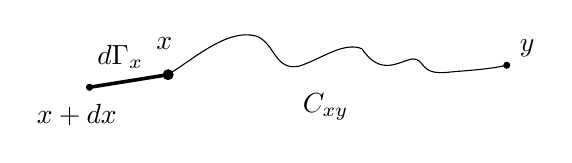
\begin{tikzpicture}[x=1cm,y=1cm]
\draw[line width=1.3pt] (0,0)--(1,0.16);
\fill (0,0) circle (0.045);
\fill (1,0.16) circle (0.07);
\draw (1,0.16) .. controls (1.35,0.38) and (1.76,0.75) .. (2.12,0.65)
.. controls (2.36,0.56) and (2.35,0.2) .. (2.67,0.27)
.. controls (2.96,0.37) and (3.23,0.58) .. (3.46,0.49)
.. controls (3.7,0.13) and (3.93,0.33) .. (4.1,0.36)
.. controls (4.27,0.37) and (4.18,0.15) .. (4.55,0.19)
.. controls (4.72,0.21) and (5.04,0.22) .. (5.3,0.28);
\fill (5.3,0.28) circle (0.045);
\node at (-0.16,-0.35) {$x+dx$};
\node at (0.39,0.39) {$d\Gamma_x$};
\node at (0.95,0.55) {$x$};
\node at (3,-0.25) {$C_{xy}$};
\node at (5.56,0.49) {$y$};
\end{tikzpicture}
\end{adjustbox}
\end{center}

$d\Gamma_x$ --- контур, идущий из $x$ в $x+dx$.
\begin{equation*}
\Psi(C_{xy}+d\Gamma_x)-\Psi(C_x)
=dx_\mu\frac{\partial\Psi}{\partial x_\mu}
\tag{18}
\end{equation*}
\Unclear{GELFAND-P000902}{equation-18-contour-index}{В первом аргументе написано $C_{xy}$, во втором — $C_x$.}

--- это определение правой части (и, след., $\dfrac{\partial\Psi}{\partial x_\mu}$).

Контур дважды прох. через т. $x$: сдвигаем и начало и конец.

Для $C_{xx}$ по очереди сдвигаются начало и конец.

Сдвинем контур параллельно:
\begin{equation*}
\frac{\partial}{\partial C^{xy}_\mu}
=\frac{\partial}{\partial x_\mu}+\frac{\partial}{\partial y_\mu}
+\int_x^y dz_\alpha\frac{\delta}{\delta\sigma_{\alpha\mu}(z)}
\tag{19}
\end{equation*}
\Unclear{GELFAND-P000902}{equation-19-cancelled-index}{В левом знаменателе перед индексом $\mu$ зачёркнут другой индекс.}

(параллельный перенос контура)

Для трансляц. инвар. ф-лов получается:
\begin{equation*}
\partial_\mu=\oint dz_\nu\frac{\delta}{\delta\sigma_{\mu\nu}(z)}.
\tag{20}
\end{equation*}
(для замкн. контуров)

\SourcePage{GELFAND-P000903}{unlabelled}
В классическом случае получается
\begin{equation*}
\mathcal L=\beta\operatorname{Tr}F_{\mu\nu}^2
\tag{21}
\end{equation*}
\begin{equation*}
S=\beta\int\operatorname{Tr}F_{\mu\nu}^2\,d^4x
\tag{22}
\end{equation*}
Имеем, как известно:
\begin{equation*}
\frac{\delta S}{\delta A_\mu(x)}=\beta(\nabla_\mu F_{\mu\nu})
\tag{23}
\end{equation*}
\Unclear{GELFAND-P000903}{equation-23-index}{В знаменателе слева написано $A_\mu(x)$, справа — $\nabla_\mu F_{\mu\nu}$.}

Поэтому (15) $\Rightarrow$
\begin{equation*}
\partial_\mu\frac{\delta\Psi}{\delta\sigma_{\mu\nu}(x)}=0
\tag{24}
\end{equation*}

\begin{center}
— · —
\end{center}

Теория $SU(\infty)$ близка к точному решению

(разлож. по степеням $\dfrac{1}{n}$; реально $SU(3)$)

\underline{Выведем квантовое ур-е дв-ния.}

\underline{КТП} Рассм. $\Psi=\Psi(\underset{\text{контур}}{c},\underset{\text{поле}}{A})$

и теперь рассмотрим
\begin{equation*}
\Psi(c)=\bigl(\int\mathcal DA_\mu\,\exp(-S)\,\Psi(c,A)\bigr)
/\bigl(\int\mathcal DA_\mu\,\exp(-S)\bigr)
\tag{25}
\end{equation*}

Квантовое ур-е дв-ния: св-во интеграла
\begin{equation*}
\int\mathcal DA_\mu(x)\frac{\delta}{\delta A_\mu(x)}
\{e^{-S}Q[A]\}\equiv0
\tag{26}
\end{equation*}

$Q[A]$ --- произв. ф-л.

Из (26) следует, что
\begin{equation*}
\left\langle\frac{\delta S}{\delta A_\mu(x)}Q\right\rangle
=\left\langle\frac{\delta Q}{\delta A_\mu(x)}\right\rangle
\qquad\text{(ур-е Швингера)}
\tag{27}
\end{equation*}

Отсюда, опуская $Q$, получим, вводя $\hbar$:
\begin{equation*}
\frac{\delta S}{\delta A_\mu(x)}
=\hbar\frac{\delta}{\delta A_\mu(x)}
\underset{\mathrm{def}}{=}\text{\Unclear{GELFAND-P000903}{equation-28-operator}{J под шляпкой}}
\tag{28}
\end{equation*}

Или:

левая часть $\overset{\text{классич.}}{\text{ур-я}}$ дв-ния заменяется варьированием по полю.

\Unclear{GELFAND-P000903}{lower-cancelled-word}{Зачёркнутое слово: неразборчиво.}
Поля $\Psi$ не независимы (много лишней информации).

$(15')\Rightarrow$
\begin{equation*}
\begin{aligned}
\beta\,\partial_\mu\frac{\delta\Psi}{\delta\sigma_{\mu\nu}}
&=\beta\left\langle\operatorname{Tr}\nabla_\mu F_{\mu\nu}\,
 p\exp\int_x^x A\,dy\right\rangle=\\
&=\left\langle\operatorname{Tr}\frac{\delta}{\delta A_\mu(x)}
 p\exp(\int_x^x A\,dy)\right\rangle,
\qquad\beta=\hbar^{-1}.
\end{aligned}
\tag{29}
\end{equation*}

\SourcePage{GELFAND-P000904}{5}
Здесь
\begin{equation*}
\Psi(c,A)=\operatorname{Tr}p\exp\left(\oint_c A\,dx\right)\tag{30}
\end{equation*}
\textit{[Зачёркнуто: $\oint_c dy$.]}
\begin{equation*}
\begin{aligned}
\frac{\delta}{\delta A_{\mu}^{jk}(x)}
\bigl(p\exp\bigl(\int_x^x A\,dy\bigr)^{kj}
&=\\
&=\oint_c dy_{\nu}\,
U^{\text{\Unclear{GELFAND-P000904}{equation31-matrix-index}{ii}}}(c_{xy})
U^{kk}(c_{yx})\delta^4(x-y),
\end{aligned}\tag{31}
\end{equation*}
\Unclear{GELFAND-P000904}{equation31-unmatched-parenthesis}{В (31) внешняя открывающая скобка не имеет видимой закрывающей.}
\Unclear{GELFAND-P000904}{equation31-cancelled}{Над знаком интеграла зачёркнут отдельный знак.}

(32) где $U$ — матрица переноса
\Unclear{GELFAND-P000904}{transfer-cancelled}{зачёркнутый знак},
$U(C_{xy})=P\exp\int_x^y A\,dx$
\begin{equation*}
\delta^4(x-y)=\frac{\delta A(y)}{\delta A(x)}
\end{equation*}
\begin{center}
\begin{adjustbox}{max width=\linewidth}
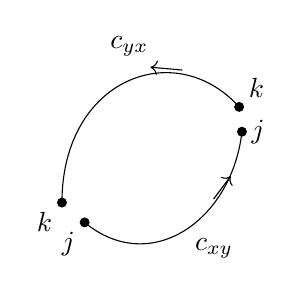
\begin{tikzpicture}[scale=0.9]
\draw (1.5,1.1) .. controls (0.6,2.1) and (-1.0,1.5) .. (-1.0,-0.25);
\draw[->] (0.7,1.62) -- (0.25,1.66);
\draw (-0.68,-0.53) .. controls (0.25,-1.3) and (1.4,-0.5) .. (1.54,0.75);
\draw[->] (1.14,-0.2) -- (1.38,0.12);
\fill (1.5,1.1) circle (2pt);
\fill (-1.0,-0.25) circle (2pt);
\fill (-0.68,-0.53) circle (2pt);
\fill (1.54,0.75) circle (2pt);
\node[above right] at (1.5,1.1) {$k$};
\node[below left] at (-1.0,-0.25) {$k$};
\node[below left] at (-0.68,-0.53) {$j$};
\node[right] at (1.54,0.75) {$j$};
\node[above] at (-0.05,1.67) {$c_{yx}$};
\node[below right] at (0.74,-0.62) {$c_{xy}$};
\end{tikzpicture}
\end{adjustbox}
\end{center}

Для произв. группы (полупростой):
\begin{equation*}
\sum_a\operatorname{Tr}\bigl(T^aU(c_{xy})T^aU(c_{yx})\bigr)
=\underbrace{\operatorname{Tr}U(c_{xy})\operatorname{Tr}U(c_{yx})
+\underset{\substack{\Vert\\-\frac{1}{N}\operatorname{Tr}(UU).}}{O\left(\frac{1}{N}\right)}}_{\text{это справа в (31) для }U(N).}
\tag{33}
\end{equation*}
Отсюда следует, что
\begin{equation*}
\beta\,\partial_{\mu}\frac{\delta\langle\Psi\rangle}{\delta\sigma_{\mu\nu}}
=\oint dy_{\nu}\,\delta^4(x-y)
\langle\Psi(c_{xy})\Psi(c_{yx})\rangle\tag{34}
\end{equation*}
Не получ. замкнутых уравнений.

$c_{xy},c_{yx}$ — замкнуты из-за $\delta^4(x-y)$

На самом деле это 1-е ур-е цепочки многопетлевых
ур-й (одной петли недостаточно) для ф-й Грина.

\Unclear{GELFAND-P000904}{contour-cancelled}{Зачёркнуто: «Не…».}
Нужно рассм. и самопересеч. контура
\begin{adjustbox}{max width=\linewidth}
\begin{tikzpicture}[scale=0.4,baseline=0pt,rotate=45]
\draw (0,0) .. controls (-0.9,0.7) and (-1.0,-0.5) .. (0,0)
.. controls (1.5,0.8) and (1.4,-0.85) .. (0,0);
\end{tikzpicture}
\end{adjustbox}
(в них вся информ. о взаимодействии)

Попытка регуляризовать $\delta$-ф-ю для придания смысла лишает
ур-е смысла (контура размыкаются) — надо делать это одноврем. с
замык. контуров.
\begin{equation*}
\langle\Psi(c_1)\Psi(c_2)\ldots\Psi(c_n)\rangle
=\langle\Psi(c_1)\rangle\langle\Psi(c_2)\rangle\ldots
\langle\Psi(\text{\Unclear{GELFAND-P000904}{equation35-argument}{$c_n$}})\rangle+O(N^{-2})\tag{35}
\end{equation*}
$\Psi=\operatorname{Tr}U(c);\quad\Psi(0)=N.$
Надо переопределить: $\Psi=N\bar\Phi$.

Для $\bar\Phi$ получается нек-рое ур-е, из к-рого получается
\underline{\underline{confinement}}

\Unclear{GELFAND-P000904}{bottom-cancelled-word}{Зачёркнутое слово под последней строкой.}
\Unclear{GELFAND-P000904}{bottom-cancelled-mark}{Отдельная густо зачёркнутая запись внизу.}

\SourcePage{GELFAND-P000905}{unlabelled}

\underline{\underline{28.1.80.}} \qquad \underline{\underline{Сем. Гельфанда.}}

\underline{А. Зелевинский.} \qquad
\underline{О раб. Каждана–Люстига}, предст. гр. Кокстера и пр.

% Имена авторов подчёркнуты волнистой линией.
\underline{D. Kazhdan, G. Lusztig}, Inv. Math, \underline{53}, $N=2$, 1979

$W$ — гр. Кокстера, $S$ — простые отражения

$W$ порождена образ. $S$ (конечное
\Unclear{GELFAND-P000905}{definition-cancelled}{нечитаемый зачёркнутый знак}
мн-во).

\begin{equation*}
W=\langle S\mid s^2=e,\;
\underset{\substack{\vert\\\text{для нек-рых пар.}}}{(ss')^{m(s,s')}=e}\rangle
\tag{1}
\end{equation*}

Группа Кокстера — это гр. с такими обр. и
\Unclear{GELFAND-P000905}{definition-relations-abbrev}{соот.}

\underline{Примеры:}

1) $S_n$: \qquad $S=\{(i,i+1)\}$
\begin{equation*}
((i,i+1)(i+1,i+2))^3=e.
\end{equation*}
все ост. явл. следствиями этих.

2) гр. Вейля $W$ сист. пр. корней

% Слово «приведённое» подчёркнуто волнистой линией.
\begin{equation*}
w=s_1\ldots s_\ell
\qquad \text{\underline{приведённое}, если \underline{длина} минимальна}
\tag{2}
\end{equation*}
\begin{equation*}
\ell=\ell(w)
\end{equation*}

Если выкинуть у привед. разл. любое подмн-во сомн., а ост. перемножить,
то получим (def) мн-во элементов $\underline{\underline{{}<w}}$

\begin{equation*}
\underline{w'=s_1\ldots\hat s_{i_1}\ldots
\hat s_{\text{\Unclear{GELFAND-P000905}{deletion-last-index}{$i_k$}}}
\ldots s_\ell<w}
\tag{3}
\end{equation*}

Это не зависит от прив. разложения.

\begin{equation*}
\mathcal A=\mathbb Z[q^{1/2},q^{-1/2}]
\end{equation*}

% Заголовок подчёркнут волнистой линией.
\underline{Алгебра Гекке:}

$\underset{\substack{\Vert\\\mathcal H_W}}{\mathcal H}$ — алгебра над
$\mathcal A$ с образующими $T_s$, $s\in S$ и соотношениями:

\begin{equation*}
(T_s+1)(T_s-q)=0,\quad \forall s
\tag*{$(4)_1$}
\end{equation*}

\begin{equation*}
\underbrace{T_sT_{s'}T_sT_{s'}\ldots}_{m(s,s')}
=\underbrace{T_{s'}T_sT_{s'}T_s\ldots}_{m(s,s')}
\tag*{$(4)_2$}
\end{equation*}
\Unclear{GELFAND-P000905}{equation4-right-mark}{справа отдельный знак, похожий на правую фигурную скобку}

$\underline{q=1}$ $\Rightarrow$ получ. групповая алгебра группы Кокстера, т.к. соотн. (1)
запис. в виде

\begin{equation*}
\underbrace{ss'ss'\ldots}_{m(s,s')}
=\underbrace{s's\ldots}_{m(s,s')}
\quad\text{\Unclear{GELFAND-P000905}{equation5-cancelled}{зачёркнутый знак}}
\tag{5}
\end{equation*}

$q$ — число элем. конечн. поля; $G$ — гр. Шевалле над $q$,

$B$ — борел. подгруппа
\begin{equation*}
\text{(}\underset{\text{матр.}}{\text{верхнетреуг.}}\text{)}
\end{equation*}

\begin{equation*}
\Rightarrow\quad
\underset{\text{(2-стор. инв. ф-и}}{\mathcal H(G,B)}
\cong\mathcal H\otimes C.
\end{equation*}

\SourcePage{GELFAND-P000906}{8}

Строится базис в алг. $\mathcal H$ (над $\mathcal A$)

Естеств. базис:

\begin{equation*}
\underset{\text{прив.}}{w=s_1\ldots s_\ell}
\rightsquigarrow
\underset{\text{(не зависит от предст.)}}{T_w=T_{s_1}\ldots T_{s_\ell}}
\tag{6}
\end{equation*}
\Unclear{GELFAND-P000906}{basis-sublinear-mark}{под словом «зависит» небольшой в-подобный знак}

$\{T_w\}$ — базис в $\mathcal H$ (хорошо изв.)

\Unclear{GELFAND-P000906}{involution-cancelled}{зачёркнуто, возможно «По»}

% Слово «инволюцию» и две следующие формулы подчёркнуты волнистой линией.
\begin{equation*}
\text{\underline{Опр.} \underline{инволюцию}}\quad
\overline{\phantom{T}}\quad\text{в }\mathcal H:\qquad
\underline{\overline{q^{1/2}}=q^{-1/2},\qquad
\bar T_w=T_{w^{-1}}^{-1}}
\bigl(\underset{\mathrm{def}}{=}(T_{w^{-1}})^{-1}\bigr).
\tag{7}
\end{equation*}

Обратимость следует из ур-я $(4)_1$:
\begin{equation*}
T_s^2+T_s(1-q)=q,\quad\text{откуда}
\end{equation*}
\begin{equation*}
T_s^{-1}=q^{-1}(T_s+1-q)
\tag{8}
\end{equation*}

Положим:
\begin{equation*}
\varepsilon_w=(-1)^{\ell(w)},\qquad q_w=q^{\ell(w)}
\tag{9}
\end{equation*}

\underline{Теорема 1.1.} $\forall w\in W,\;\exists!\;C'_w\in\mathcal H:$

\begin{equation*}
(1)\quad\overline{C'_w}=C'_w
\tag{10}
\end{equation*}

\begin{equation*}
(2)\quad C'_w=q_w^{-1/2}\sum_{y\le w}P_{y,w}\cdot T_y,
\tag{11}
\end{equation*}
где
\begin{equation*}
P_{w,w}=1,\qquad
\underset{(y<w)}{P_{y,w}}\text{ — полином от }q\text{ с коэфф. в }\mathbb Z
\text{ степени }\le\frac12(\ell(w)-\ell(y)-1)
\tag{12}
\end{equation*}

\begin{align*}
\bar T_s&=q^{-1}T_s+q^{-1}-1\\
\overline{q^{-1/2}T_s}&=q^{-1/2}T_s+q^{-1/2}-q^{1/2}\\
\underbrace{\overline{q^{-1/2}T_s+q^{-1/2}}}_{C'_s}
&=q^{-1/2}T_s+q^{-1/2}
\end{align*}

Или: $P_{s,s}=1,\quad
P_{\text{\Unclear{GELFAND-P000906}{example-overwritten-index}{e}},s}=1.$

% Заголовок «Гипотеза» подчёркнут волнистой линией.
\underline{Гипотеза:} Пусть $g$ — компл. полупр. алгебра Ли, $W$ — гр. Вейля;

\begin{equation*}
M_w\text{ — модуль Верма};\qquad
[M_w:L_y]=
P_{\text{\Unclear{GELFAND-P000906}{multiplicity-nested-indices}{$w_0w,w_0y$}}}
\underset{\substack{\backslash\\\text{знач. в точке 1}}}{(1)}
\quad\text{— \underline{\underline{гипотеза}}}
\tag{13}
\end{equation*}

$L_w$ — единств. неприв. фактор, \qquad $L_y,\;y\le w$

Для $\operatorname{GL}(4)$ проверено.

Были даны несколько эквив. переформулировок.

\begin{equation*}
P_{y,w}=\sum_{i\ge0}q^i\dim\operatorname{Ext}^{\ell(w)-\ell(y)-2i}(M_y,L_w)
\tag{14}
\end{equation*}
или
\begin{equation*}
\operatorname{Ext}^j(M_y,L_w)=0,\quad\text{если }j\;
\begin{adjustbox}{max width=\linewidth}
\begin{tikzpicture}[baseline=-0.5ex,x=1ex,y=1ex]
\draw (-0.5,0.35)--(0.5,0.35);
\draw (-0.5,0)--(0.5,0);
\draw (-0.5,-0.35)--(0.5,-0.35);
\draw (-0.2,-0.75)--(0.2,0.75);
\end{tikzpicture}
\end{adjustbox}
\;\ell(w)-\ell(y)\pmod{2}
\tag{15}
\end{equation*}

Положим:
\begin{equation*}
C_w=\varepsilon_wj(C'_w),\quad\text{где }j(q^{1/2})=q^{-1/2},\quad
j(T_w)=\varepsilon_wq_w^{-1}T_w
\tag{16}
\end{equation*}
\begin{center}
($j$ — вспом. инволюция)
\end{center}

\SourcePage{GELFAND-P000907}{unlabelled}
\begin{equation*}
y\prec w\overset{\mathrm{def}}{\Longleftrightarrow}y<w,\quad
\varepsilon_y=-\varepsilon_w,\quad
\operatorname{deg}P_{y,w}=\frac12\bigl(l(w)-l(y)-1\bigr).
\tag{17}
\end{equation*}
Обозначим тогда
\begin{equation*}
\mu(y,w)\quad\text{старший коэффициент }P_{y,w}.
\end{equation*}
\underline{Теорема 1.3.} $s\in S$, $v\in W\Rightarrow$
\begin{equation*}
T_sC_v=\begin{cases}
-C_v,\quad sv<v,\\
qC_v+q^{1/2}C_{sv}+q^{1/2}\displaystyle\sum_{\substack{z<v\\sz<z}}\mu(z,v)C_z
\end{cases}
\tag{18}
\end{equation*}
\begin{center}
если $sv>v$
\end{center}
(Явно выписано действие образующих на базисе)

Отсюда удаётся разложить рег. предст. (блочно треуг. вид).

\underline{\underline{B. Mc Pherson}} (?)
\Unclear{GELFAND-P000907}{speaker-cancelled-initial}{зачёркнутая буква перед фамилией}
\underline{\underline{Макферсон}}.

\Unclear{GELFAND-P000907}{speaker-parenthesis}{(Bol)}

Геом. интерп. $P_{s,t}(q)$

— $q$ полин. Пуанкаре странных когомологий клеток Шуберта.

Группы $IH_i(X)$ — intersection-
\Unclear{GELFAND-P000907}{english-cancellation}{зачёркнуто перед homologie}
homologie groups (для мн-зий с
\Unclear{GELFAND-P000907}{singularity-cancellation}{зачёркнутый знак}
особ.)

(опред. докладчиком)

\underline{св-ва их:}

\begin{equation*}
1)\quad X\text{ }\text{\Unclear{GELFAND-P000907}{nonsingularity-abbreviation}{несинг.}}\quad\Rightarrow\quad IH_i(X)=H_i(X)
\tag{1}
\end{equation*}
\begin{equation*}
2)\quad IH_i(X)\times IH_{n-i}(X)\longrightarrow
\mathbb Q^{\text{\Unclear{GELFAND-P000907}{pairing-superscript}{v}}}
\quad\text{при }\dim X=n.
\tag{2}
\end{equation*}
Топологич. простейшее опрд.

\begin{equation*}
\underset{\text{комплексное}}{X}=X_n\supset X_{n-2}\supset X_{n-4}\supset\cdots\supset X_0
\tag{3}
\end{equation*}
\begin{center}стратификации\end{center}
\underline{Условия:}

а) $X_i-X_{i-2}$ — мн-зие, неособое, разм. $i$.

б) вдоль $X_{i-2}$ [вписано над строкой: окрестность]
топологически трив. (локально) в точках $X_{i-2}-X_{i-4}$.

\begin{equation*}
\underset{\substack{\text{(замкн.)}\\\text{разм. }n}}{X\text{ — шуберт. кл.}}
\quad\Rightarrow\quad\text{меньшие клетки годятся для стратифик.}
\end{equation*}
Тогда по опрд.

\Unclear{GELFAND-P000907}{definition-cancelled-symbol}{зачёркнуто: I}

\begin{equation*}
IH_i(X)\underset{\mathrm{def}}{=}
\left\{\frac{\begin{gathered}
i\text{-циклы, встр. каждое }X_{n-2c}\\
\text{по мн-ву размерности }i-c-1
\end{gathered}}{\begin{gathered}
\partial\text{ от }i+1\text{ цепей, пересек. каждое }X_{n-2c}\\
\text{по мн-ву разм. }i-c
\end{gathered}}\right.
\tag{4}
\end{equation*}
\underline{Теорема:} (с пом. спец. теории когом.
\Unclear{GELFAND-P000907}{theorem-manifolds-abbreviation}{мн-зий}
хар-ки $p$)

\begin{equation*}
P_{s,t}(q)=q^{\text{\Unclear{GELFAND-P000907}{polynomial-prefactor-exponent}{?}}}
\sum_i\dim IH_i(X_t,X_t-y_s)q^i.
\tag{5}
\end{equation*}
$s,t$ — элем. группы Вейля;

$y_s$ — точка на меньшей кл. Шуберта ($s$-й).

\SourcePage{GELFAND-P000908}{unlabelled}
\underline{\underline{4.2.80.}} \underline{сем. Гельфанда}

\underline{Г. Ольшанский.}

\begin{equation*}
G=\mathrm{GL}(\infty,\mathbb R)=\bigcup_{n\ge1}\mathrm{GL}(n,\mathbb R)
\tag{1}
\end{equation*}
\begin{equation*}
K=\mathrm{SO}(\infty)=\bigcup_{n\ge1}\mathrm{SO}(n)
\tag{2}
\end{equation*}
$\exists$ сем-во предст. $G$, для к-рых $K$ играет роль max комп. подгр.

\begin{equation*}
T_{\pi_1,s_1,\ldots,\pi_k,s_k},\qquad
\pi_i\in O(n_i)^{\wedge},\quad s_i\in\mathbb R.
\tag{3}
\end{equation*}
\Unclear{GELFAND-P000908}{restriction-cancelled-word}{зачёркнуто: Огр}
огранич. на $K$ имеет конечнокр. дискр. спектр.

Аналог. вар. для $U(\infty)$.

\begin{equation*}
\mathrm{SO}(p,\infty)=\overline{\bigcup_{n\ge1}\mathrm{SO}(p,n)}
\tag{4}
\end{equation*}
\begin{equation*}
U(p,\infty)=\overline{\bigcup_{n\ge1}U(p,n)}
\tag{5}
\end{equation*}
\begin{equation*}
\mathrm{Sp}(p,\infty)=\overline{\bigcup_{n\ge1}\mathrm{Sp}(p,n)}
\tag{6}
\end{equation*}
\begin{center}(пополнения)\end{center}
(4)–(6) — группы типа I и
\Unclear{GELFAND-P000908}{classification-abbreviation}{дан.}
описание всех неприв. представлений.

\underline{\underline{Mc Pherson.}}

\underline{о раб. Габриэлова, Гельфанда, Лосика} о комбин. классах Понтрягина,
к-рую он понимает лучше авторов.

(о 1-м классе)

$X$ — симплиц. 4-мн-зие

($X$ — симпл. комплекс
\Unclear{GELFAND-P000908}{complex-final-glyph}{g}:

\begin{equation*}
\forall\text{ симплекса }\sigma\quad\exists\text{ отобр.}\quad
\text{\Unclear{GELFAND-P000908}{mapping-cancelled-symbol}{зачёркнутый знак}}
\quad\psi:\underset{\text{звезда }\sigma}{\operatorname{St}\sigma}\longrightarrow\mathbb R^4,
\tag{1}
\end{equation*}
гомеоморфное вблизи внутренности $\sigma$, линейное на каждом симплексе.

\underline{Идеи иллюстр. на 2-мн-зии.}

\SourceFigure{GELFAND-P000908}{star-illustration}{Слева пространственно изображённая сетка с верхней, левой, нижней и двумя правыми вершинами; левая и передняя рёбра обведены жирно, есть тонкие прерывистые внутренние отрезки. У выделенной передней части стоит $\sigma$. Из этой части вправо идёт изогнутая стрелка с надписью $\psi$. Справа ромб из двух треугольников с общей горизонтальной стороной.}

(опред. $\operatorname{St}$)

$H$ (гиперсимплекс)
\qquad $C$ — (конфигурационное пр-во) — термины.

\begin{equation*}
\begin{adjustbox}{max width=\linewidth}
\begin{tikzcd}
H \arrow[d,"\text{клеточное отобр.}"] & C \arrow[d,"\text{клеточное отобр.}"] \\
X & X^D
\end{tikzcd}
\end{adjustbox}
\tag{2}
\end{equation*}
$X^D$ — двойств. клет. разбиение (звёздное).

Клеточность: остов $\longrightarrow$ остов.

\begin{equation*}
\begin{adjustbox}{max width=\linewidth}
\begin{tikzcd}
\Gamma \arrow[r,phantom,"\subset"] \arrow[d] & H\times_X C \arrow[dl] \\
X' &
\end{tikzcd}
\end{adjustbox}
\tag{3}
\end{equation*}

\SourcePage{GELFAND-P000909}{13}
будет постр. $\widetilde P$ — коцикл в $C^4(\Gamma)$.

\begin{equation*}
\pi^*\underset{\text{рац. класс Понтрягина}}{p^1(X)}=[\widetilde P].
\tag{4}
\end{equation*}
\underline{Конструкция.}

\underline{\underline{$H$}}

$\forall$ симпл. $\sigma$ в $X$ строим многогранник $H\sigma$ из отображений
\begin{equation*}
\{\text{вершины звезды }\sigma\}\overset{h}{\longrightarrow}[0,1].
\tag{5}
\end{equation*}
\begin{equation*}
\text{(6)}_1\qquad1)\quad h(v)=1\quad\text{при }v\in\sigma
\end{equation*}
\begin{equation*}
\text{(6)}_2\qquad2)\quad\sum_v h(v)=5=4+1.\qquad(=\dim+1)
\end{equation*}
\underline{Примеры.}

а) \underline{симпл. высшей разм.}\qquad $\underline{\operatorname{St}\sigma=\sigma}$

\begin{adjustbox}{max width=\linewidth}
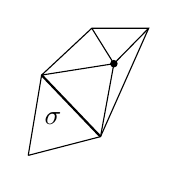
\begin{tikzpicture}[scale=0.85]
\coordinate (a) at (0,0);
\coordinate (b) at (0.2,1.2);
\coordinate (c) at (0.95,1.9);
\coordinate (d) at (1.8,1.9);
\coordinate (e) at (1.08,0.28);
\coordinate (f) at (1.28,1.37);
\draw (a)--(b)--(c)--(d)--(e)--(a);
\draw (b)--(f)--(c) (f)--(d) (f)--(e);
\draw[thick] (b)--(e);
\fill (f) circle (1.6pt);
\node at (0.37,0.55) {$\sigma$};
\end{tikzpicture}
\end{adjustbox}
\qquad $H\sigma=1$ точка (всюду 1 должны быть ф-и).

б) симпл. коразм. 1.

\begin{adjustbox}{max width=\linewidth}
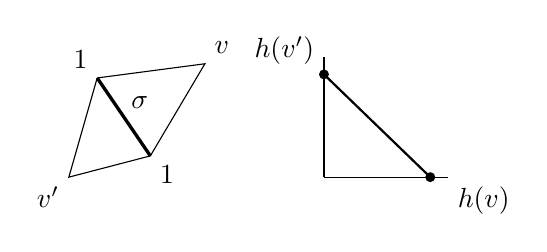
\begin{tikzpicture}[scale=0.9]
\coordinate (a) at (0.4,1.4);
\coordinate (b) at (1.15,0.3);
\coordinate (v) at (1.92,1.6);
\coordinate (vp) at (0,0);
\draw (a)--(v)--(b)--(vp)--(a);
\draw[very thick] (a)--(b);
\node[above left] at (a) {$1$};
\node[below right] at (b) {$1$};
\node[above right] at (v) {$v$};
\node[below left] at (vp) {$v'$};
\node at (1.0,1.05) {$\sigma$};
\draw (3.6,0)--(3.6,1.7) (3.6,0)--(5.35,0);
\draw[thick] (3.6,1.45)--(5.1,0);
\fill (3.6,1.45) circle (2pt);
\fill (5.1,0) circle (2pt);
\node[above left] at (3.6,1.45) {$h(v')$};
\node[below right] at (5.35,0) {$h(v)$};
\end{tikzpicture}
\end{adjustbox}
\qquad $H\sigma$ — отрезок.

Так происходит и в общем случае.

в) \underline{Коразмерность 2.}

в$'$) (простой случай)

\begin{adjustbox}{max width=\linewidth}
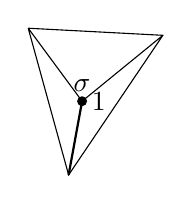
\begin{tikzpicture}[scale=0.9]
\coordinate (a) at (0,1.75);
\coordinate (b) at (1.9,1.65);
\coordinate (c) at (0.57,-0.32);
\coordinate (s) at (0.76,0.72);
\draw (a)--(b)--(c)--(a) (a)--(s)--(b);
\draw[thick] (s)--(c);
\fill (s) circle (2pt);
\node[above] at (s) {$\sigma$};
\node[right] at (s) {$1$};
\end{tikzpicture}
\end{adjustbox}

\SourceFigure{GELFAND-P000909}{cube-section}{Перспективное изображение куба с тонкими сплошными и прерывистыми внутренними рёбрами. На трёх вершинах стоят жирные точки; их соединяет выделенная жирная ломаная от верхней дальней левой вершины через верхнюю переднюю правую к дальней нижней правой. Между её звеньями и диагональю видна штриховка. Слева вертикальная стрелка с $h(v')$, наклонная вправо-вверх стрелка с $h(v'')$, снизу горизонтальная стрелка вправо с $h(v)$.}

$H\sigma$ — симплекс. (2-мерный симплекс)

в$''$)

\begin{adjustbox}{max width=\linewidth}
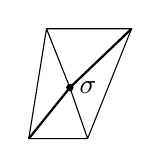
\begin{tikzpicture}[scale=0.9]
\coordinate (a) at (0.25,1.55);
\coordinate (b) at (1.45,1.55);
\coordinate (c) at (0.83,0);
\coordinate (d) at (0,0);
\coordinate (s) at (0.58,0.72);
\draw (a)--(b)--(c)--(d)--(a) (a)--(s)--(c);
\draw[thick] (d)--(s)--(b);
\fill (s) circle (1.5pt);
\node[right] at (s) {$\sigma$};
\end{tikzpicture}
\end{adjustbox}

Рассечём 4-мерный куб
\Unclear{GELFAND-P000909}{cube-trailing-mark}{нижний знак, похожий на 2}
плоскостью,
\Unclear{GELFAND-P000909}{octahedron-cancelled-label}{зачёркнуто: abc}
\Unclear{GELFAND-P000909}{equidistant-abbreviation}{равноотст.}
от верт. (каких-то)

\SourceFigure{GELFAND-P000909}{small-octahedron}{Небольшое перспективное изображение октаэдра: верхняя, левая, нижняя, правая и передняя вершины соединены видимыми рёбрами; задние соединения частично прерывисты. Верхняя передняя треугольная часть обведена жирно, у правой вершины короткие поперечные штрихи.}

— октаэдр.

\SourceFigure{GELFAND-P000909}{labelled-octahedron}{Крупный октаэдр справа. У верхней вершины надпись $abc$, у левой $ace$, у правой $abd$, у нижней $ade$, у передней средней $acd$, внутри слева $abe$. Внешний контур и передние рёбра сплошные, часть внутренних соединений прерывиста. Верхнее ребро к передней вершине и поперечное ребро слева к ней выделены жирно.}

Метки в вершинах многогранников.

Вершины — ф-и, прин. только знач. 0 и 1.

Индексы — те вершины, где 1.

\begin{equation*}
H\sigma\times\sigma\qquad
\sigma<\sigma'\quad\Rightarrow\quad H(\sigma')<H(\sigma)
\quad\text{(звёзды так вложены)}
\end{equation*}
отсюда есть общая часть

\begin{equation*}
H\sigma\times\sigma\quad\text{и}\quad H\sigma'\times\sigma',\quad\text{а именно}
\end{equation*}
\begin{equation*}
\underline{H\sigma'\times\sigma}
\end{equation*}
Склеиваем по этой общей части.

Получается пр-во $H$.

\Unclear{GELFAND-P000909}{bottom-cancelled-word}{зачёркнуто: Построим}


\SourcePage{GELFAND-P000910}{unlabelled}
\underline{Построение $C$.}

$C\sigma$ строим сначала.

По опр. сущ. отображение (хотя бы одно)
\begin{equation*}
\operatorname{st}\sigma\overset{\psi}{\longrightarrow}\mathbb R^4,\tag{7}
\end{equation*}
удовл. условиям, к-рые были перечисл. выше.

$C\sigma$ — мн-во всех таких $\psi$

Пусть $\sigma$ имеет коразмерность $k$.
$(=$ [зачёркнутый или переписанный знак:
\Unclear{GELFAND-P000910}{codimension-overwriting}{1 или неразобранный знак}] $4-k)$

$\psi$ общего полож., если все мн-ва
\begin{equation*}
\left\{
\underbrace{v_1\ldots v_i}_{\text{все верш. }\sigma}
\quad
\underbrace{v'_1\ldots v'_k}_{k\text{ верш. из }\operatorname{st}\sigma\setminus\sigma}
\right\}\tag{8}
\end{equation*}
(всего 5 точек)

общего положения в $\mathbb R^4$.

$\psi$ имеет особенность (speciality) $c$, если $\exists c$
[к $c$ снизу приписано: \Unclear{GELFAND-P000910}{speciality-insertion}{набор или незав.}]
[зачёркнуто: \Unclear{GELFAND-P000910}{speciality-cancelled-glyph}{и}]
мн-ва, для к-рых это
[зачёркнуто: \Incomplete{GELFAND-P000910}{cancelled-before-condition}{Зачёркнутое слово перед «условие» не удалось прочесть.}]
условие \underline{не выполнено}.

Неизвестно; стратификация или клет. разбиение.

\underline{Пример:}

\SourceFigure{GELFAND-P000910}{configuration-examples}{Слева пятиугольник с пятью отмеченными вершинами, внутренней точкой с подписью $\sigma$ и отрезками от неё к вершинам. Горизонтальная стрелка направлена вправо к меньшему пятиугольнику с внутренними отрезками; справа от него подчёркнуто $c=0$. Ниже расположены ещё два пятиугольника с подчёркнутыми подписями $c=1$ и $c=2$. В среднем выделены наклонный отрезок от нижней левой вершины через внутреннюю точку к правой верхней вершине и другие внутренние отрезки; слева внизу виден слабый наклонный штрих, продолжающийся внутрь фигуры. В нижнем две диагонали пересекаются внутри, к пересечению подходит дополнительный отрезок от левой вершины. Точные соединения, слабый наклонный штрих и степень выделения линий требуют проверки по оригиналу.}

[Справа от рисунка $c=0$:]
($\sigma$ и 2 другие верш. не лежат на одной пр.)

\underline{$C\sigma$ для точек $(k=4)$}

$C\sigma$ — 1 точка для каждой связной компон. конфигур.
общего положения

(дискр. пр-во из точек)

\underline{$C\sigma$ для ребер $(k=3)$}

$C\sigma$ будет графом

$C\sigma\ni$ по точке для $\forall$ св. компон.
[сверху вписано: невыр.] конфигур.

\underline{1 ребро для каждой св. компоненты пр-ва конфиг. с особ. 1}

$c=1\Rightarrow\exists$ ровно 2 способа прив. их в общее полож.

\begin{center}
\begin{adjustbox}{max width=\linewidth}
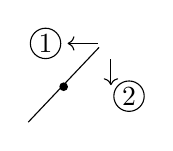
\begin{tikzpicture}[x=1cm,y=1cm]
\draw (-0.45,-0.45)--(0.45,0.5);
\fill (0,0) circle (0.055);
\draw[->] (0.43,0.55)--(0.05,0.55);
\node[draw,circle,inner sep=1pt] at (-0.23,0.55) {1};
\draw[->] (0.6,0.35)--(0.6,0.02);
\node[draw,circle,inner sep=1pt] at (0.83,-0.12) {2};
\end{tikzpicture}
\end{adjustbox}
\end{center}

Петель нет
(\tikz[baseline=-2pt]{\draw (0,0) .. controls (0.05,0.65) and (0.75,0.65) .. (0.48,0.3) .. controls (0.3,0.13) and (0.05,0.03) .. (0,0);\fill (0,0) circle (0.04);}).

\SourcePage{GELFAND-P000911}{14}
\underline{Граф связен} (трудная теорема!)

$\underline{k=2}\Rightarrow$ 2 мерный (не симпл.) комплекс.

точки \Unclear{GELFAND-P000911}{points-line-stroke}{длинное тире или зачёркнутый фрагмент}
для св. комп. конфиг. общ. полож.

ребра для конфиг. с особ. 1

квадрат для св. комп. —〃— 2

\SourceFigure{GELFAND-P000911}{square-two-diagonals}{Наклонный четырёхугольник с обеими диагоналями и подчёркнутой подписью $c=2$ снизу. Слева отдельно стоит узкий двойной наклонный штрих; неясно, является ли он самостоятельным знаком, зачёркиванием или частью рисунка. У диагоналей стрелок не видно.}

ломаем каждую 2-мя способами

— это стороны квадрата.

\begin{equation*}
\left.\begin{gathered}k=1,\\k=2\end{gathered}\right\}
C\sigma\underset{\mathrm{def}}{=}1\text{ точка.}
\end{equation*}
\Unclear{GELFAND-P000911}{repeated-k-two}{Во второй строке написано $k=2$.}

(все конфигур. общего полож. и сост. связное мн-во)

\begin{center}
\begin{adjustbox}{max width=\linewidth}
\begin{tikzcd}
C\arrow[d] & C\sigma\times\sigma^D\arrow[d] \\
X^D & \sigma^D
\end{tikzcd}
\end{adjustbox}
\end{center}
[Справа:] естеств. образом склеиваются?

\SourceFigure{GELFAND-P000911}{simplex-dual-figure}{Фигура из нескольких треугольных областей с верхней, левой, правой, внутренней и нижней вершинами. Через верхнюю левую область и её внутреннюю границу проходит утолщённый отрезок с двумя отмеченными концами; над ним подписи $\sigma$ и $\sigma^D$. Правая внутренняя диагональ и часть рёбер слабы или прерывисты. Точная инцидентность отрезка, меток и слабых рёбер требует проверки по оригиналу.}

\begin{equation*}
\begin{gathered}
\sigma^D\subset\sigma'^D\\
\sigma\supset\sigma'
\end{gathered}
\end{equation*}

Тогда есть отобр.

\begin{equation*}
\text{конфиг. для }\sigma\longleftarrow\text{конфиг. для }\sigma'
\end{equation*}
[Справа:] (звезда \Unclear{GELFAND-P000911}{star-abbreviation}{ширящ. или шириц.})

(ограничение отображений $\psi$)

\begin{equation*}
C\sigma\longleftarrow C\sigma'
\end{equation*}

Имеем отображение:

\begin{center}
\begin{adjustbox}{max width=\linewidth}
\begin{tikzcd}
H\underset{X}{\times}C\arrow[d]\\
X'
\end{tikzcd}
\end{adjustbox}
\end{center}
[Справа:] $X'=X$ разб. на пересеч. симплексов и двойств. разб.

\noindent\rule{12cm}{0.4pt}

\begin{equation*}
\Gamma\subset H\underset{X}{\times}C
\end{equation*}

$\Gamma$ — клетки из $H$ (грани гиперсимплекса)

вершине $\leadsto$ точка конфиг. в общем полож. $\Rightarrow$ тогда
включаем прямые произв. в $\Gamma$

$\sigma$ — симпл. из $X$

$H\sigma\qquad C\sigma$

\underline{грани $H\sigma$}
$\Unclear{GELFAND-P000911}{bottom-relation}{\simeq}$
[зачёркнуто: \Incomplete{GELFAND-P000911}{cancelled-before-five}{Короткое зачёркнутое слово перед «пятерка» (возможно, «грань») не удалось надёжно прочесть.}]
пятерка точек $\overset{\psi}{\longrightarrow}$ пятерку;
если общего полож., то включ. в $\Gamma$

[От $\psi$ наклонная выноска: соотв. грань $C\sigma$.]

[На правом поле, с изогнутой стрелкой от нижней записи о $\Gamma$:
зачёркнуто \Unclear{GELFAND-P000911}{margin-cancelled-glyph}{с или неразобранный знак};
произв., ниже \underline{прямое}.]

\SourcePage{GELFAND-P000912}{unlabelled}

\begin{equation*}
\pm\frac{1}{48}\widetilde P
\qquad \text{над точками }X
\end{equation*}

Рассмотрим 4-мерн. грань
[над строкой вставлено: (гиперсимпл.); под вставкой:
\Unclear{GELFAND-P000912}{top-insertion-mark}{неразборчиво}]
сост. из следующих отобр.
\begin{equation*}
h:\{\text{верш. звезды }\sigma\}\longrightarrow[0,1]
\end{equation*}
\begin{equation*}
h=1\text{ на }\sigma
\end{equation*}

$h=1$ на 3-х вершинах (других), на 5 переменна, на остальных $=0$
\begin{equation*}
(9)\qquad
\begin{gathered}
\text{другие}\\
\text{возм.}
\end{gathered}
\left\{
\begin{array}{rclc}
2&\rule{3.4cm}{0.3pt}&5&\rule{4.4cm}{0.3pt}\\
1&\rule{3.4cm}{0.3pt}&5&\rule{4.4cm}{0.3pt}\\
0&\rule{3.4cm}{0.3pt}&5&\rule{4.4cm}{0.3pt}
\end{array}
\right.
\end{equation*}

(нет других 4-мерных граней)

\begin{equation*}
\widetilde P=0\quad .\ \text{на }
\Unclear{GELFAND-P000912}{zero-face-label}{(9)_1}
\text{ и }(9)_4
\end{equation*}
\begin{equation*}
\widetilde P=\pm\frac{1}{48}
\quad\text{на }(9)_2\text{ и }(9)_3.
\end{equation*}

Число относится ориентир. клетке.

Ориент. грани $(9)_2$ отвеч. \underline{чётности упоряд. 5 точек.}

\begin{center}
\begin{adjustbox}{max width=\linewidth}
\begin{tikzpicture}[x=1cm,y=1cm]
\node at (-0.95,0.85) {\fbox{$(9)_2$}};
\node at (0.90,1.22) {\underline{5 вект.}};
\node at (2.00,0.70) {в $R^4$};
\draw[->] (0,0) -- (-0.16,0.58);
\draw[->] (0,0) -- (0.55,1.03);
\draw[->] (0,0) -- (1.56,0.46);
\draw[->] (0,0) -- (0.94,-0.17);
\draw (0,0) -- (0.09,-0.48);
\node[anchor=west] at (3.80,0.35)
  {На $\sigma$ и \underline{2 точки} натянута плоскость};
\draw (4.51,0.18) -- (4.51,-0.02);
\node[anchor=west] at (4.29,-0.20) {вершина};
\draw (6.14,0.10) -- (6.14,-0.15);
\node[anchor=west] at (6.05,-0.44) {слева в $(9)_2$};
\draw[->] (0.45,-0.55) -- (0.37,-1.05);
\node[anchor=west] at (0.80,-0.80) {проекц. вдоль плоскости};
\draw[->] (4.97,-0.80) -- (5.64,-0.66);
\draw[->] (-0.07,-2.18) -- (-0.40,-1.79);
\draw[->] (-0.07,-2.18) -- (0.22,-1.61);
\draw[->] (-0.07,-2.18) -- (0.62,-1.61);
\draw[->] (-0.07,-2.18) -- (0.99,-1.71);
\draw[->] (-0.07,-2.18) -- (0.97,-2.19);
\node[anchor=west] at (1.14,-1.85) {--- в $R^2$};
\end{tikzpicture}
\end{adjustbox}
\end{center}

10 ориентаций плоскости (каждая пара)

Надо взять $(-1)^i\frac{1}{48}$, где $i$ --- число
\underline{положит.} ориентаций

(неважно, кто $>0$, т.к. всего 10)

\fbox{$(9)_3$}\qquad то же самое

получ. 5 векторов в $R^3$,

тоже 10 ориент. в \underline{$R^3$} и \underline{т.д.}

$G_{2,2}(R)$ --- 2-мерн. плоск. в $R^4$

есть 6 [зачёркнуто:
\Unclear{GELFAND-P000912}{schubert-cancelled-word}{циклов};
\Incomplete{GELFAND-P000912}{schubert-cancelled-word}{Зачёркнутое слово прочитано не полностью.}
Над строкой вставлено: Замыкания клеток] Шуберта

в $R^4$:
[зачёркнуто: \Unclear{GELFAND-P000912}{coordinate-cancelled-symbol}{неразборчиво}]
6 коорд. 2-мерн. плоскостей

Плоск.,
[зачёркнуто: \Unclear{GELFAND-P000912}{transverse-cancelled-symbol}{неразборчиво};
вставлено: не]
трансверс. данной коорд. плоскости

\textquotedblleft\underline{enhanced} projective configur. of 4 points in
\Unclear{GELFAND-P000912}{enhanced-projective-dimension}{$RP^2$}\textquotedblright

\textquotedblleft improved --- улучшенные

\begin{center}
\begin{adjustbox}{max width=\linewidth}
\begin{tikzpicture}[x=1cm,y=1cm]
\draw (0,0) -- (-0.43,0.08);
\draw (0,0) -- (0.55,0.48);
\draw (0,0) -- (-0.09,-0.72);
\draw (0,0) -- (0.24,-0.58);
\node[anchor=west] at (1.30,0.23)
  {\underline{4 луча из 0 в $R^2$}};
\end{tikzpicture}
\end{adjustbox}
\end{center}

(4 [зачёркнуто:
\Incomplete{GELFAND-P000912}{rays-cancelled-word}{Зачёркнутое слово неразборчиво.};
над строкой вставлено: точки]
в $RP^1$ ---
\Unclear{GELFAND-P000912}{unenhanced-word}{неулучш.},
здесь лучи)

\SourcePage{GELFAND-P000913}{15}

\begin{equation*}
L\subset R^4,\qquad \dim L=2
\end{equation*}

в $R^4/L$ есть 4 луча!!

Надо взять их ангарм. отношение

2 таких набора эквив., если они перев. действием $GL(2,R)$

\begin{center}
\begin{adjustbox}{max width=\linewidth}
\begin{tikzcd}
G_{2,2}(R)\arrow[d,"\pi"]\\
\begin{gathered}
\text{классы эквив.}\\
\text{улучш. 4-к.}
\end{gathered}
\end{tikzcd}
\end{adjustbox}
\end{center}

$P$ --- 4-форма, предст. понтр. класс

\begin{center}
\begin{adjustbox}{max width=\linewidth}
\begin{tikzpicture}[x=1cm,y=1cm]
\node at (0,0) {$\pi_*(P)=d\Phi$};
\draw (1.03,-0.16) -- (1.15,-0.42);
\node[anchor=west] at (1.25,-0.57) {ф-я (дилогарифм)};
\end{tikzpicture}
\end{adjustbox}
\end{center}

\begin{center}
\begin{adjustbox}{max width=\linewidth}
\begin{tikzcd}
\xi\arrow[d]\\
G_{2,2}(R)
\end{tikzcd}
\end{adjustbox}
\end{center}

$P=P(\xi)$,\qquad $\xi$ --- 2-мерное (станд.) рассл. на $G_{2,2}(R)$

стр. какая-то связность.

\SourcePage{GELFAND-P000914}{unlabelled}

\underline{\underline{11.2.80 г.}}\qquad
\underline{Сем. Гельфанда.}

\underline{\underline{R. Mc Pherson.}}

Грассманиан $G_{n,k}$ из $n$-плоскостей в $R^{n+k}$,

(неориентированных)

\underline{Идея}:

Элементу $G_{n,k}$ соотв. пара

гиперсимплекс $+$ конфигурация

$\widetilde C_{n,k}=$
[зачёркнуто:
\Incomplete{GELFAND-P000914}{configuration-cancelled-words}{Два зачёркнутых слова неразборчивы.}]
оснащ. проект. конфигурации

[под «оснащ.»:] enhanced

$n+k$ точек в $k$-мерном пр-ве
(или в (\Unclear{GELFAND-P000914}{projective-dimension}{$k+1$})-мерн. проектив.)

\Incomplete{GELFAND-P000914}{lower-clipped-fragments}{Ниже последней полной строки видны только обрезанные верхние штрихи; чтение невозможно.}

\SourcePage{GELFAND-P000915}{unlabelled}
% Верхняя часть исходного кадра свободна от рукописного текста.
\underline{18. 2. 80 г.}\qquad \underline{Сем. Гельфанда}

\underline{Захаров}\quad \underline{В. Е.}

\underline{Ур-я Бенни}

\SourceFigure{GELFAND-P000915}{surface-diagram}{Схема поверхности над горизонтальным дном: сплошная волнистая линия с двумя подъёмами, горизонтальный штриховой отрезок под правым гребнем, вертикальный отрезок от дна к поверхности. Над поверхностью стоит h; над правым гребнем — неуверенно читаемый знак l, L или i. Слева стрелка вверх с подписью z, справа стрелка вниз и g = 1.}

$h$ — форма поверхности, $h=h(\Unclear{GELFAND-P000915}{horizontal-coordinate}{\vec r},t)$.

$\Unclear{GELFAND-P000915}{horizontal-coordinate}{\vec r}$ — вектор в плоскости дна

$\vec u=\vec u(\Unclear{GELFAND-P000915}{horizontal-coordinate}{\vec r},z,t)$ — скорость в плоскости дна

$w$ — вертик. скорость

идеальная несжим. жидкость

\begin{equation*}
\frac{\partial w}{\partial z}+\operatorname{div}\vec u
=\Unclear{GELFAND-P000915}{continuity-zero}{0}
\end{equation*}

[На правом поле:]
Бенни — прибл. ур-е.
\underline{длинные волны}
$(w\ll u)$

\begin{equation*}
\frac{\partial w}{\partial t}
+\underbrace{(u\nabla)w+w\frac{\partial w}{\partial z}}_{\text{пренебрегаем по ср. со след. членами}}
\Unclear{GELFAND-P000915}{pressure-sign}{-}\frac{\partial p}{\partial z}+1=0
\end{equation*}

\SourcePage{GELFAND-P000916}{unlabelled}
\begin{equation*}
(1)\quad\left\{
\begin{aligned}
\frac{\partial w}{\partial z}+\operatorname{div}\vec u
&=\Unclear{GELFAND-P000916}{equation-zeros}{0}\\
\vec u_t+(u\nabla)u+w\frac{\partial\vec u}{\partial z}+\nabla h
&=\Unclear{GELFAND-P000916}{equation-zeros}{0}
\end{aligned}
\right.
\end{equation*}

\begin{equation*}
\frac{\partial p}{\partial z}+1=\Unclear{GELFAND-P000916}{equation-zeros}{0}
\quad\Longrightarrow\quad
p=-z+h(\Unclear{GELFAND-P000916}{pressure-coordinate}{\vec r},t)
\end{equation*}

\begin{equation*}
(1)_3\quad\left\{h_t+\operatorname{div}\int_0^h\vec u\,dz
=\Unclear{GELFAND-P000916}{equation-zeros}{0}\right.
\end{equation*}

$(1)$ — система ур-й Бенни

Манин [снизу вписано: и др.] — 1-мерный случай.

\underline{Захаров}: а) в 1-мерном случае
\Unclear{GELFAND-P000916}{zakharov-first-verb}{вывел}
счёт. з.с. \Unclear{GELFAND-P000916}{zakharov-second-verb}{пок.}, их независимость

б) другая гам. структура (более простая)

в) что-то для 2-мерной зав. (с гамильтоновостью)

Идея: \Unclear{GELFAND-P000916}{idea-word}{переинтерпрет.} задачи.

\underline{И.М.Г.}\quad \underline{Коллективные дифф. ур-я:}

когда частицы не взаимод.
\Unclear{GELFAND-P000916}{interaction-abbreviation}{неп.}, но
[зачёркнуто: \Incomplete{GELFAND-P000916}{cancelled-word}{Зачёркнутое короткое слово не удалось прочесть.}]
[над зачёркнутым вписано: \Unclear{GELFAND-P000916}{inserted-words}{заряжены и}]
вместе созд. поле, к-рое
[между строками: (\Unclear{GELFAND-P000916}{parenthetic-field}{физическ. поле})]
действ. на каждую в отдельности.
\Unclear{GELFAND-P000916}{last-clause}{След. раздел за обыкн.}
дифф. ур-ями.
% Нижняя часть исходного кадра свободна от рукописного текста.

\SourcePage{GELFAND-P000917}{unlabelled}
\underline{22.9.80г.}\qquad \underline{Сем. Гельфанда.}

\underline{Фукс.} Есть мн-ие с особ. (алгебр., компл.) и есть стратификация.
\begin{equation*}
(1)\quad X=X_{2n}\supset X_{2n-2}\supset
\Unclear{GELFAND-P000917}{filtration-indices}{X_{n-3}\supset X_{n-4}}\supset\ldots
\end{equation*}
$X_i\setminus X_{i-1}$ — $i$-мерное мн-ие.

Около данного страта всё устроено одинаково (вся окрестность).

Рассм. сингул. симплексы пр-ва $X$, облад. нек-рыми доп. св-вами.
\begin{equation*}
\sigma_j\qquad \dim\sigma_j=j
\end{equation*}
[Между $\dim$ и $\sigma_j$ зачёркнуто:
\Unclear{GELFAND-P000917}{dimension-cancellation}{неразборчивый знак}.]
\begin{equation*}
(2)\quad
\Unclear{GELFAND-P000917}{dimension-condition}{\dim(\sigma_j\cap X_{2n-i})=j-2i}
\end{equation*}
В этих когом. есть двойств. Пуанкаре. Это другие когомологии.

\underline{Пример:} Две 2-мерн. сферы, склеенные в
\Unclear{GELFAND-P000917}{example-gluing}{1-й точке}
\SourceFigure{GELFAND-P000917}{two-spheres-contact}{Справа от примера два горизонтальных замкнутых овальных контура без подписей; левый немного шире, правый расположен чуть выше. В узкой области их соприкосновения или пересечения видны утолщённые повторные штрихи. Точное устройство этой области требует проверки по оригиналу.}

Эти когомологии \underline{не гомотопически инвариантны}.

\underline{Обычные гомологии.}
\begin{equation*}
\left\{\begin{array}{ll}
0 & \mathbb{Z}\\
1 & 0\\
2 & \mathbb{Z}+\mathbb{Z}
\end{array}\right.
\end{equation*}
[Справа от верхней строки зачёркнуто:
\Unclear{GELFAND-P000917}{ordinary-homology-cancellation}{неразборчиво}.]

Они не удовл. двойств. Пуанкаре (видно сразу).

\underline{Гом. Макферсона}
\begin{equation*}
\left\{\begin{array}{ll}
0 & \mathbb{Z}+\mathbb{Z}\\
1 & 0\\
2 & \mathbb{Z}+\mathbb{Z}
\end{array}\right.
\end{equation*}

\begin{center}
\begin{adjustbox}{max width=\linewidth}
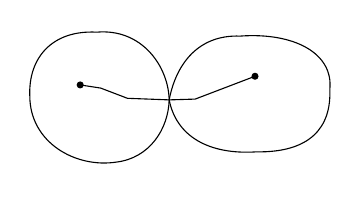
\begin{tikzpicture}[x=1cm,y=1cm]
\draw (1.80,0) .. controls (1.79,0.43) and (1.45,0.91) .. (0.88,0.86)
 .. controls (0.31,0.89) and (0.01,0.53) .. (0.03,0.05)
 .. controls (0.03,-0.54) and (0.61,-0.87) .. (1.13,-0.79)
 .. controls (1.55,-0.74) and (1.79,-0.37) .. (1.80,0);
\draw (1.80,0) .. controls (1.89,0.47) and (2.18,0.83) .. (2.70,0.81)
 .. controls (3.39,0.86) and (3.89,0.59) .. (3.84,0.13)
 .. controls (3.86,-0.36) and (3.58,-0.67) .. (2.91,-0.66)
 .. controls (2.30,-0.70) and (1.89,-0.46) .. (1.80,0);
\draw (0.67,0.19) -- (0.93,0.15) -- (1.27,0.02) -- (1.80,0)
 -- (2.13,0.01) -- (2.89,0.30);
\fill (0.67,0.19) circle (0.045);
\fill (2.89,0.30) circle (0.045);
\end{tikzpicture}
\end{adjustbox}
\end{center}
Такой симплекс \underline{запрещается}.

\underline{Гипотеза:} совпадают с $L_2$-когомологиями.

(этим \underline{интересовался Борель})

Пусть есть ровно одна изолир. особенность. Тогда MF-когом.
[Под «MF-когом.»: (Макферс.)]
\begin{equation*}
\left.\begin{aligned}
\underline{\text{в разм.}}\ >\frac{\dim X}{2}\quad&\text{совп. с обычными,}\\
\underline{\text{в разм.}}\ <\frac{\dim X}{2}\quad&\text{из двойств. Пуанкаре.}
\end{aligned}\right]\quad\text{это опр. Делиня}
\end{equation*}

\SourcePage{GELFAND-P000918}{unlabelled}
Опр. Делиня в более общей ситуации (индуктивное)

\underline{М.И. Граев.}

Из работ Гельф.-Гинд.-\Unclear{GELFAND-P000918}{reference-author-abbreviation}{Шап.}
\begin{equation*}
\begin{array}{ll}
\text{ФА} & 13:2\\
\text{ФА} & 14:4
\end{array}
\end{equation*}

$\mathcal{D}\subset\mathbb{R}^n$;

$(n+k-1)$-пар. сем-во кривых
[Перед «-пар.» зачёркнуто:
\Unclear{GELFAND-P000918}{family-parameter-cancellation}{неразборчивый знак};
$(n+k-1)$ вписано над строкой и обведено линией, ведущей к зачёркнутому знаку.]
\begin{equation*}
x_i=\varphi_i(x_1,\xi),\quad
\xi=(\xi_1,\ldots,\Unclear{GELFAND-P000918}{parameter-vector-length}{\xi_n}),\quad \xi\in\Gamma
\end{equation*}

Интегр. преобр.
\begin{equation*}
\xi=(\xi_1,\ldots,\xi_{n+k-1});
\end{equation*}
$f(x),\quad \operatorname{supp}f\subset\mathcal{D}$
\begin{equation*}
F(\xi)=I_\chi f
=\int f(x_1,\Unclear{GELFAND-P000918}{integral-first-index}{\varphi_1}(x_1,\xi),\ldots,
\varphi_n(x_1,\xi))\chi(x_1,\xi)\,dx_1
\end{equation*}
[Справа над формулой, со стрелкой к $\chi$: фикс всюд. ф-я $>0$.]

Интересно найти такие мн-ия кривых, для к-рых
$\exists$ лок. формула обращ. (восст. по инт. по кривым, прох. через
эту точку или беск. близкую)

Такое мн-ие кривых наз. \underline{допустимым}.

$\forall x^0\in\mathcal{D}$ опр. оператор
$F(\xi)\to\Unclear{GELFAND-P000918}{differential-operator-glyph}{\mathcal{H}}_{x^0}F$
\begin{equation*}
\Gamma_{x^0}\qquad
x_i^0=\varphi_i(\Unclear{GELFAND-P000918}{fixed-point-coordinate-index}{x_i^0},\xi)
\qquad \dim\Gamma_{x^0}=k
\end{equation*}
[Под $x$ в индексе левого $\Gamma$ зачёркнуто:
\Unclear{GELFAND-P000918}{gamma-subscript-cancellation}{неразборчивый знак}.]

$\Unclear{GELFAND-P000918}{differential-operator-glyph}{\mathcal{H}}_{x^0}$ — дифф. форма на
\begin{equation*}
\Unclear{GELFAND-P000918}{differential-operator-glyph}{\mathcal{H}}_{x^0}F
=\sum a_{ij}(x_1^0,\xi)\frac{\partial F}{\partial\xi_j}\,d\xi_i
+F\sum b_i(x_1^0,\xi)\,d\xi_i.
\end{equation*}
Оператор $\Unclear{GELFAND-P000918}{differential-operator-glyph}{\mathcal{H}}_{x^0}$
наз. \underline{допустимым}, если $\forall$ ф-и $f$ дифф. форма
$\Unclear{GELFAND-P000918}{differential-operator-glyph}{\mathcal{H}}_{x^0}I_\chi f$
явл. замкнутой.

$k>1\ \Rightarrow$ это полное опред.

Если $k=1$, то автоматич. замкнута и треб., чтобы ф-л
\begin{equation*}
f\mapsto\int
\Unclear{GELFAND-P000918}{differential-operator-glyph}{\mathcal{H}}_{\Unclear{GELFAND-P000918}{base-point-zero-position}{x_0}}I_\chi f
\end{equation*}
был сосредоточен в т. $x_0$.

Тривиальный ф-л:
$\underline{\Unclear{GELFAND-P000918}{differential-operator-glyph}{\mathcal{H}}_{x^0}F=d(\mu F)}$

Важен фактор по трив. ф-лам.



\end{document}
